% conceitos basicos
Neste capítulo faremos uma apresentação dos conceitos básicos
necessários para o entendimento e desenvolvimento deste trabalho. Na
seção \ref{sec:defin} mostraremos as definições usadas no decorrer
deste trabalho. As seções \ref{sec:rev}, \ref{sec:trans}
e \ref{sec:rev_trans} descrevem, respectivamente, os problemas de
ordenação por reversões, ordenação por transposições e ordenação por
reversões e transposições.

\section{Definições}
\label{sec:defin}
Para todos os problemas usamos as seguintes definições.

\textit{Permutação.} 
Para fins computacionais, um genoma é representado por uma $n$-tupla
de genes, e quando não há genes repetidos essa $n$-tupla é chamada de
permutação. Uma permutação é representada como $\pi =
(~\pi_{1}~\pi_{2}~\ldots~\pi_{n}~)$, para $\pi_{i} \in \mathbb{N}$, $0
< \pi_{i} \leq n$ e $i \neq j \leftrightarrow \pi_{i} \neq \pi_{j}$. A
permutação identidade é representada como $\iota =
(~1~2~3~\ldots~n~)$. Para a demonstração dos eventos, usaremos como
base a permutação $\pi = (~4~7~3~6~2~5~1~)$.

\textit{Eventos de rearranjo.}
Os eventos de rearranjo tratados neste trabalho são os eventos de
transposição e reversão quando ocorrem isoladamente e quando ocorrem
de forma conjunta. Os eventos são representados por $\rho$ e são
aplicados a $\pi$ de uma maneira específica.

\section{Ordenação por Reversões}
\label{sec:rev}
Um evento de reversão ocorre quando um bloco do genoma é
invertido. Uma reversão $\rho(i, j)$, para $1 \leq i < j \leq n$,
aplicada ao genoma $\pi = (~\pi_{1}~\pi_{2}~\ldots~\pi_{n}~)$ gera a
permutação $\rho\pi =
(\pi_{1}~\ldots~\pi_{i-1}~\pi_{j}~\pi_{j-1}~\ldots~\pi_{i+1}$
$\pi_{i}~ \pi_{j+1}~\ldots~\pi_{n})$, caso a orientação de $\pi$ não é
conhecida (Figura \ref{fig:rev_nao_orientada}), e $\rho\pi =
(\pi_{1}~\ldots~\pi_{i-1}~-\pi_{j}~-\pi_{j-1}~\ldots~-\pi_{i+1}$
$-\pi_{i}~ \pi_{j+1}~\ldots~\pi_{n})$, caso a orientação de $\pi$ é
conhecida (Figura \ref{fig:rev_orientada}). 

\begin{figure}
  \centering
  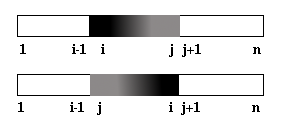
\includegraphics{images/rev_nao_orientada.png} 
  \caption{Reversão em uma permutação não orientada.}
  \label{fig:rev_nao_orientada}
\end{figure}

\begin{figure}
  \centering
  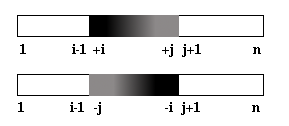
\includegraphics{images/rev_orientada.png}
  \caption{Reversão em uma permutação orientada.}
  \label{fig:rev_orientada}
\end{figure}

A distância de reversão $d_{r}(\pi,\sigma)$ entre duas permutações
$\pi$ e $\sigma$ é o número mínimo $r$ de reversões $\rho_{1}$,
$\rho_{2}$, $\ldots$, $\rho_{r}$ tal que
$\pi \rho_{1} \rho_{2} \ldots \rho_{r} = \sigma$. Note que a distância
de reversão entre $\pi$ e $\sigma$ é igual à distância de reversão
entre $\sigma^{-1} \pi$ e $\iota$. Então, sem perda de generalidade,
podemos dizer que o problema da distância de reversão é equivalente ao
problema de ordenação por reversões, que é a distância de reversão
entre a permutação $\pi$ e a permutação identidade $\iota$, denotado
por $d_{r}(\pi)$.

Em um estudo inicial sobre este problema, Bafna e
Pevzner \cite{BafnaPevzner*1996} apresentaram um algoritmo de
aproximação com razão de 1.5 quando a orientação de genes é conhecida
e 1.75 caso contrário.

Conhecer a orientação dos genes em um genoma é um fator importante no
problema de reversão, pois existem algoritmos polinomiais para o caso
em que a orientação é conhecida. No caso em que não se conhece a
orientação dos genes o problema de encontrar a distância de reversão
pertence a classe dos problemas NP-Difíceis \cite{Caprara*1997}.

O primeiro algoritmo polinomial para o problema de reversão com
orientação conhecida foi criado por Hannenhalli e Pevzner
\cite{HannenhalliPevzner*1995} que fez uso de várias operações
aplicadas a uma estrutura intermediária conhecida como grafo
de \bkp{}. A estratégia usada por Hannenhalli e Pevzner foi
simplificada no trabalho de Bergeron \cite{Bergeron*2005}. Atualmente
já existe um algoritmo com complexidade sub-quadrática
\cite{TannierSagot*2004} e, quando apenas a distância é necessária, um
algoritmo linear pode ser usado \cite{BaderMoretYan*2001}.

Um resultado importante obtido por Meidanis, Walter e Dias
\cite{MeidanisWalterDias*2000}, mostrou que toda teoria sobre
reversões desenvolvida para genomas lineares pode ser adaptada
facilmente para genomas circulares, que são comuns em seres inferiores
como vírus e bactérias.

Quando a orientação dos genes não é conhecida existem algoritmos de
aproximação que seguiram a ideia do trabalho de Bafna e Pevzner citado
anteriormente como, por exemplo, o algoritmo implementado por Berman,
Hannenhalli e Karpinski \cite{BermanHannenhalliKarpinski*2002} com
razão de aproximação de 1.375.

\subsection{Grafo de \bkp{}}
\label{subsec:rev_bkp}
O conceito de grafo de \bkp{} foi introduzido no trabalho de Bafna e
Pevzner \cite{BafnaPevzner*1996}. Inicialmente a permutação $\pi$ é
estendida adicionando o elemento $\pi_{0} = 0$ e $\pi_{n+1} =
n+1$. Dois elementos consecutivos $\pi_{i}$ e $\pi_{i+1}$, $0 \le
i \le n$, são \textit{adjacentes} quando $|\pi_{i} - \pi_{i+1}| = 1$,
e são \estr{breakpoints} caso contrário. Define-se um grafo de arestas
coloridas $G(\pi)$ com $n + 2$ vértices \{0, 1, $\ldots$, $n$, $n +
1$\}. Unimos os vértices $i$ e $j$ com uma aresta preta se $(i, j)$
for um \estr{breakpoint}. Unimos os vértices $i$ e $j$ com uma aresta
cinza se $|i - j| = 1$ e $i$, $j$ não são consecutivos em
$\pi$. Denotamos por $b_r(\pi)$ o número de \bkp{} existentes em
$\pi$. A Figura \ref{fig:rev_grafo_bkp} mostra o grafo de \bkp{} para
a permutação $\pi = (~4~7~3~6~2~5~1~)$.

\begin{figure}[h]
  \centering 
  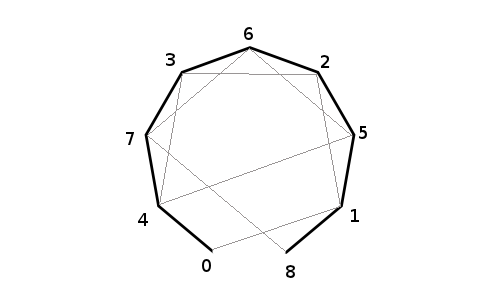
\includegraphics[scale=0.5]{images/rev_grafo_bkp.png} 
  \caption{Grafo de \bkp{} para a permutação $\pi = (~4~7~3~6~2~5~1~)$.}
  \label{fig:rev_grafo_bkp}
\end{figure}

\subsection{Limitantes}
\label{subsec:rev_limitantes}
Para o problema de ordenação por reversões usamos dois tipos de limitantes:

\begin{itemize}
\item{\textit{rev\_def}. 
Este é o limitante padrão, com limite inferior igual à 0 e limite
superior igual a $n$ (tamanho da permutação).}
\item{\textit{rev\_br}
Usando o conceito de \bkp{}, temos que uma reversão atua em dois
pontos em uma permutação e, portanto, pode reduzir o número de \bkp{}
em pelo menos um e no máximo dois \cite{BafnaPevzner*1996}, levando ao
Teorema \ref{teo:rev_bound}.

\begin{teo}
\label{teo:rev_bound}
Para qualquer permutação $\pi$, $\frac{b_r(\pi)}{2} \leq d_r(\pi) \leq
  b_r(\pi)$.
\end{teo}}
\end{itemize}

\section{Ordenação por Transposições}
\label{sec:trans}

Um evento de transposição ocorre quando dois blocos adjacentes no
genoma trocam de posição.

TODO

\section{Ordenação por Reversões e Transposições}
\label{sec:rev_trans}
TODO
